\documentclass{article}
\usepackage[utf8]{inputenc}
\usepackage[T1]{fontenc}
\usepackage{amsmath}
\usepackage{amssymb}
\usepackage[fixamsmath,disallowspaces]{mathtools}
\usepackage{colortbl}
\usepackage{tikz}
\usetikzlibrary{shapes.geometric,positioning}

\begin{document}

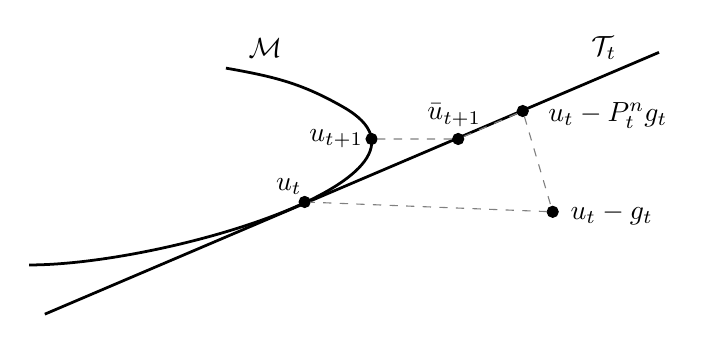
\begin{tikzpicture}
    
    \node (M) at (1.0,2.75) {$\mathcal{M}$};
    \draw[line width = 1pt]  (0.5,2.5) to[out=350,in=150] (2,2)  to[out=-30,in=0]  (-2,0);
    
    \draw[line width = 1pt,-] (-1.8,.-0.625) -- (6., 2.7);
    \node at (5.3, 2.75) {$\mathcal{T}_t$};
    
    \node[inner sep=1, outer sep=1] (u_t) at (1.5,0.8) {};
    \filldraw (u_t) circle (2pt);
    \node at (1.3,1.) {$u_t$};
    \node[inner sep=1, outer sep=1] (utpproj) at (3.45, 1.6) {};
    \filldraw (utpproj) circle (2pt);
    \node at (3.4, 1.9) {$\bar{u}_{t+1}$};
    \node[inner sep=1, outer sep=1] (utp) at (2.35, 1.6) {};
    \filldraw (utp) circle (2pt);
    \node at (1.9, 1.6) {$u_{t+1}$};
    \node[inner sep=1, outer sep=1] (utpexact) at (1.5 + 4.2*0.75, 0.9  -.3*0.75) {};
    \node at (5.4, 0.65) {$u_t - g_t$};
    \filldraw (utpexact) circle (2pt);
    \node[inner sep=1, outer sep=1] (utpn) at (1.12 + 4.2*0.75, 2.18  -.3*0.75) {};
    \filldraw (utpn) circle (2pt);
    \node at (5.35, 1.9) {$u_t - P^n_t g_t$};
    
    

    % projection/recompression lines

    \draw[dashed, gray] (utp) -- (utpproj) -- (utpn) -- (utpexact) -- (u_t);


    % density plot



\end{tikzpicture}

\end{document}